\themaG
\graphicspath{{../Ch6_Se_reperer_sur_un_plan_et_dans_l_espace/Images/}}

\chapter{Se repérer}
\label{C06}


%%%%%%%%%%%%%%%%%%%%%%%%%%%%%%%%%%%%%%%%%%
\begin{prerequis}[Connaissances et compétences abordées]
   \begin{itemize}
      \item Se repérer sur un plan ou sur une carte (école, quartier, ville, village).
      \item Divers modes de représentation de l’espace : maquettes, plans, schémas.
   \end{itemize}
\end{prerequis}

\vfill

\begin{debat}[Débat : le GPS] 
   GPS est l'acronyme de l'anglais \og Global Positioning System \fg{}, qui signifie \og système de positionnement global\fg. Le système comprend au moins vingt-quatre satellites émetteurs, et un nombre quasi-illimité de récepteurs. Le récepteur GPS calcule les informations émises par quatre satellites au minimum, pour obtenir les coordonnées en longitude, latitude, et altitude du point où il se trouve. Il permet de situer de manière assez précise un objet ou un personnage sur la Terre. Actuellement, la plupart des téléphones portables possèdent un GPS.
   \flushright{\footnotesize\it Source : Wikidia, l'encyclopédie des 8-13 ans}
   \begin{center}
      \begin{pspicture}(0,-0.3)(5,4.2)
         \psset{linewidth=1mm}
         \pscircle[linecolor=A1](2,2){1}
         \pscircle[linecolor=B1](3.7,1.5){1}
         \pscircle[linecolor=J1](3,3){1}
         \psline[linewidth=0.4mm,arrowsize=0.5]{->}(0,3)(2.95,2.05)
         \rput(-1,3){Je suis là !}
      \end{pspicture}
   \end{center}
   \begin{cadre}[B2][F4]
      \begin{center}
         Vidéo : \href{https://www.youtube.com/watch?v=WoqpQbWdacQ}{\bf Comment fonctionne un GPS}, chaîne YouTube {\it Unisciel}, série {\it Kezako}.
      \end{center}
   \end{cadre}
\end{debat}

\vfill

\textcolor{PartieGeometrie}{\large\sffamily\bfseries Cahier de compétences} : chapitre 1, exercices 1, 18, 20, 21, 23, 37, 40, 41, 42. 


%%%%%%%%%%%%%%%%%%%%%%%%%%%%%%%%%%%%%
%%%%%%%%%%%%%%%%%%%%%%%%%%%%%%%%%%%%%
\activites

\begin{activite}[La rose des vents]
   {\bf Objectifs :} tracer une figure géométrique précise et soignée ; suivre un programme de construction ; connaître les quatre points cardinaux.
   \begin{QCM}
         Suivre les étapes de construction de la rose des vents, la colorier, la découper et la coller dans le cours.
         {\psset{unit=0.9}
         \small
         \begin{center}
            \begin{pspicture}(-4,-4)(4,3.5)
               \psset{linewidth=0.7mm}
               \pscircle(0,0){3}
               \psline(-3,0)(3,0)
               \psline(0,-3)(0,3)
               \rput(-1.5,0.35){\ucm{3}}
               \rput(-3.7,0){\large\textcolor{B1}{\bf 1)}}
            \end{pspicture}
         \begin{pspicture}(-4,-4)(4,3.5)
            \pscircle(0,0){3}
               \psline(-3,0)(3,0)
               \psline(0,-3)(0,3)
               \psset{linewidth=0.7mm}
               \psline(3;45)(3;-135)
               \psline(3;135)(3;-45)
               \rput(-3.7,0){\large\textcolor{B1}{\bf 2)}}
            \end{pspicture}

            \begin{pspicture}(-4,-4)(4,3)
               \pscircle(0,0){3}
               \psline(-3,0)(3,0)
               \psline(0,-3)(0,3)
               \psline(3;45)(3;-135)
               \psline(3;135)(3;-45)
               \psset{linewidth=0.7mm}
               \pscircle(0,0){1}
               \pscircle(0,0){2.5}
               \rput(-0.6,0.25){\ucm{1}}
               \rput(1.5,0.25){\ucm{2,5}}
               \rput(-3.7,0){\large\textcolor{B1}{\bf 3)}}
            \end{pspicture}
            \begin{pspicture}(-4,-4)(4,3)
               \pscircle(0,0){3}
               \psline(-3,0)(3,0)
               \psline(0,-3)(0,3)
               \psline(3;45)(3;-135)
               \psline(3;135)(3;-45)
               \pscircle(0,0){1}
               \pscircle(0,0){2.5}
               \psset{linewidth=0.7mm}
               \pspolygon(0,-2.9)(1;-45)(2.9,0)(1;45)(0,2.9)(1;135)(-2.9,0)(1;-135)
               \rput(-3.7,0){\large\textcolor{B1}{\bf 4)}}
            \end{pspicture}

            \begin{pspicture}(-4,-3.3)(4,3)
               \pscircle(0,0){3}
               \psline(-3,0)(3,0)
               \psline(0,-3)(0,3)
               \psline(3;45)(3;-135)
               \psline(3;135)(3;-45)
               \pscircle(0,0){1}
               \pscircle(0,0){2.5}
               \pspolygon(0,-2.9)(1;-45)(2.9,0)(1;45)(0,2.9)(1;135)(-2.9,0)(1;-135)
               \psset{linewidth=0.7mm}
               \pspolygon(2.5;45)(0,1)(2.5;135)(-1,0)(2.5;-135)(0,-1)(2.5;-45)(1,0)
               \rput(-3.7,0){\large\textcolor{B1}{\bf 5)}}
            \end{pspicture}
            \begin{pspicture}(-4,-3.3)(4,3)
               \psset{linewidth=0.7mm}
               \pspolygon(2.5;45)(0,1)(2.5;135)(-1,0)(2.5;-135)(0,-1)(2.5;-45)(1,0)
               \pspolygon[fillstyle=solid,fillcolor=white](0,-3)(1;-45)(3,0)(1;45)(0,3)(1;135)(-3,0)(1;-135)
               \psline(-3,0)(3,0)
               \psline(0,-3)(0,3)
               \psline(2.5;45)(2.5;-135)
               \psline(2.5;135)(2.5;-45)
               \rput(-3.7,0){\large\textcolor{B1}{\bf 6)}}
            \end{pspicture}
         \end{center}}
   \end{QCM}
\end{activite}


%%%%%%%%%%%%%%%%%%%%%%%%%%%%%%%%%%%%%%
%%%%%%%%%%%%%%%%%%%%%%%%%%%%%%%%%%%%%%
\cours 

\section{Se repérer sur un quadrillage} %%%

\begin{methode*2*2}[Repérage sur un quadrillage]
Pour se repérer sur un quadrillage, on peut utiliser les {\bf coordonnées} des cases ou des n\oe uds.
   \exercice
      Quadrillage à {\bf cases}. \\
      Déterminer l'emplacement du carré et du disque. \\
      \psset{unit=0.7}
      \begin{pspicture}(-2,0)(6,6.5)
         \rput(1,1){\psgrid[gridlabels=0,subgriddiv=0](5,5)}
         \rput(1.5,0.5){A}
         \rput(2.5,0.5){B}
         \rput(3.5,0.5){C}
         \rput(4.5,0.5){D}
         \rput(5.5,0.5){E}
         \rput(0.5,0.5){\multido{\n=1+1}{5}{\rput(0,\n){\n}}}
         \pscircle[linecolor=violet,fillstyle=solid,fillcolor=violet](4.5,3.5){0.3}
         \psframe[linecolor=violet,fillstyle=solid,fillcolor=violet](2.25,4.25)(2.75,4.75)
      \end{pspicture}
   \correction
      Le carré est en B4, le disque en D3.
   \exercice
      Quadrillage à {\bf n\oe uds}. Déterminer l'emplacement du triangle et du pentagone. \\
      \psset{unit=0.7}
      \begin{pspicture}(-2,0)(6,6.5)
         \rput(1,1){\psgrid[gridlabels=0,subgriddiv=0](5,5)}
         \rput(1,0.5){A}
         \rput(2,0.5){B}
         \rput(3,0.5){C}
         \rput(4,0.5){D}
         \rput(5,0.5){E}
         \rput(6,0.5){F}
         \rput(0.5,1){\multido{\n=0+1}{6}{\rput(0,\n){\n}}}
         \psdot[linecolor=violet,linewidth=2mm,dotstyle=triangle*](3,2)
         \psdot[linecolor=violet,linewidth=1.8mm,dotstyle=pentagon*](4,6)
      \end{pspicture}
   \correction
      Triangle (C;1) et pentagone (D;5).
\end{methode*2*2}


%%%%%%%%%%%%%%%%%%%%%%%%%%%%%%%%%%%%%%%
\section{Se repérer sur un plan ou une carte}

\begin{definition}
   \begin{minipage}{8cm}
      Une {\bf rose des vents} est une figure qui indique les 4 points cardinaux : est, nord, ouest et sud et éventuellement les orientations intermédiaires.
   \end{minipage}
   \hfill
   \begin{minipage}{4cm}
      \psset{unit=0.5}
      \footnotesize
      \begin{pspicture}(-3,-4)(4,4)
         \pspolygon[fillstyle=solid,fillcolor=white](2.5;45)(0,1)(2.5;135)(-1,0)(2.5;-135)(0,-1)(2.5;-45)(1,0)
         \pspolygon[fillstyle=solid,fillcolor=white](0,-3)(1;-45)(3,0)(1;45)(0,3)(1;135)(-3,0)(1;-135)
         \psline(-3,0)(3,0)
         \psline(0,-3)(0,3)
         \psline(2.5;45)(2.5;-135)
         \psline(2.5;135)(2.5;-45)
         \rput(3.5;0){E}
         \rput(3.4;45){NE}
         \rput(3.5;90){N}
         \rput(3.4;135){NO}
         \rput(3.5;180){O}
         \rput(3.4;225){SO}
         \rput(3.5;270){S}
         \rput(3.4;315){SE}
      \end{pspicture}
   \end{minipage}
\end{definition}

\begin{center}
   \begin{minipage}{7cm}
      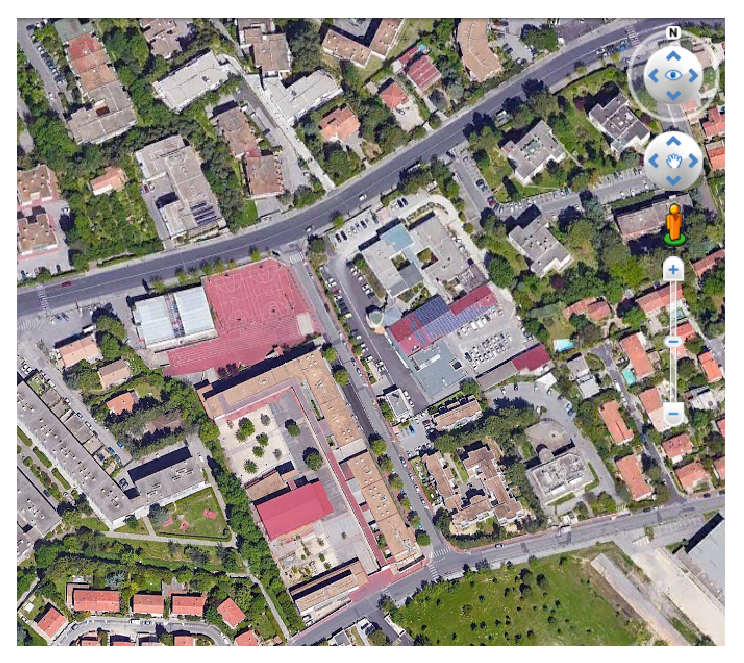
\includegraphics[width=7cm]{plan_college}
   \end{minipage}
   \qquad
   \begin{minipage}{7cm}
      Sur une carte, on peut se repérer grâce à la rose des vents, mais sur les cartes actuelles et les GPS, bien souvent, seule la direction du nord est indiquée. Elle permet à elle seule de se repérer dans le plan.
   \end{minipage}
\end{center}


%%%%%%%%%%%%%%%%%%%%%%%%%%%%%%%%%%%%%%%%%%
\exercicesbase

\begin{colonne*exercice}

\serie{Se repérer sur un quadrillage}

\begin{exercice}
   Déterminer l'emplacement des formes suivantes : \\
   \psset{unit=0.7}
   \begin{center}
      \begin{pspicture}(0,0)(8,7.5)
         \psgrid[gridlabels=0,subgriddiv=0](8,8)
         \rput(1.5,0.5){A}
         \rput(2.5,0.5){B}
         \rput(3.5,0.5){C}
         \rput(4.5,0.5){D}
         \rput(5.5,0.5){E}
         \rput(6.5,0.5){F}
         \rput(7.5,0.5){G}
         \rput(0.5,0.5){\multido{\n=1+1}{7}{\rput(0,\n){\n}}}
         \psset{linecolor=A1,linewidth=1.5mm}
         \psdot[dotstyle=triangle*](3.5,1.5)
         \psdot[dotstyle=pentagon*](4.5,6.5)
         \psdot[dotstyle=square*](1.5,2.5)
         \psdot[dotstyle=*](7.5,3.5)
         \psdot[dotstyle=diamond*](6.5,5.5)
      \end{pspicture}
   \end{center}
\end{exercice}

\begin{exercice}
   Déterminer l'emplacement des formes suivantes :  \\
   \psset{unit=0.7}
   \begin{center}
      \begin{pspicture}(0,0)(8,7.5)
         \psgrid[gridlabels=0,subgriddiv=0](1,1)(8,8)
         \rput(1,0.5){A}
         \rput(2,0.5){B}
         \rput(3,0.5){C}
         \rput(4,0.5){D}
         \rput(5,0.5){E}
         \rput(6,0.5){F}
         \rput(7,0.5){G}
         \rput(8,0.5){H}
         \rput(0.5,1){\multido{\n=0+1}{8}{\rput(0,\n){\n}}}
         \psset{linecolor=A1,linewidth=1.5mm}
         \psdot[dotstyle=triangle*](6,1)
         \psdot[dotstyle=pentagon*](2,3)
         \psdot[dotstyle=square*](1,7)
         \psdot[dotstyle=*](4,5)
         \psdot[dotstyle=diamond*](8,6)
      \end{pspicture}
   \end{center}
\end{exercice}

\begin{exercice}
   Placer les lettres suivantes dans la grille, puis vérifier en lisant de gauche à droite et de haut en bas. \\
   A $\to$ g6 ; B $\to$ b8 ; C $\to$ b4 ; E $\to$ d4 et h1 ; J $\to$ a2 ; O $\to$ h5 \\
   R $\to$ d7 ; S $\to$ b1 et f3 ; T $\to$ e1 et h3 ; U $\to$ c2 ; V $\to$ c5.
   \psset{unit=0.6}
   \begin{center}
      \begin{pspicture}(0,0)(9,9)
         \psgrid[gridlabels=0,subgriddiv=0](9,9)
         \rput(1.5,0.5){a}
         \rput(2.5,0.5){b}
         \rput(3.5,0.5){c}
         \rput(4.5,0.5){d}
         \rput(5.5,0.5){e}
         \rput(6.5,0.5){f}
         \rput(7.5,0.5){g}
         \rput(8.5,0.5){h}
         \rput(0.5,0.5){\multido{\n=1+1}{8}{\rput(0,\n){\n}}}
      \end{pspicture}
   \end{center}
\end{exercice}

\begin{exercice}
   Placer les formes suivantes dans la grille. \\
   \psset{linecolor=A1,linewidth=1.5mm}
   \hspace*{10mm} \psdot[dotstyle=*](0,0.08) \quad (d,4) \quad \psdot[dotstyle=triangle*](0,0.08) \quad (g,2) \quad \psdot[dotstyle=square*](0,0.08) \quad (a,0) \quad \psdot[dotstyle=pentagon*](0,0.08) \quad (b,6) \quad \psdot[dotstyle=diamond*](0,0.08) \quad (f,3)
   \psset{unit=0.6}
   \begin{center}
      \begin{pspicture}(0,0)(7,7)
         \psgrid[gridlabels=0,subgriddiv=0](1,1)(7,7)
         \rput(1,0.5){a}
         \rput(2,0.5){b}
         \rput(3,0.5){c}
         \rput(4,0.5){d}
         \rput(5,0.5){e}
         \rput(6,0.5){f}
         \rput(7,0.5){g}
         \rput(0.5,1){\multido{\n=0+1}{7}{\rput(0,\n){\n}}}
      \end{pspicture}
   \end{center}

\end{exercice}

\end{colonne*exercice}

\serie{Se repérer sur un plan ou une carte}

\begin{exercice}
   Voici le plan d'une cabine d'un Boeing 767.
   \begin{center}
      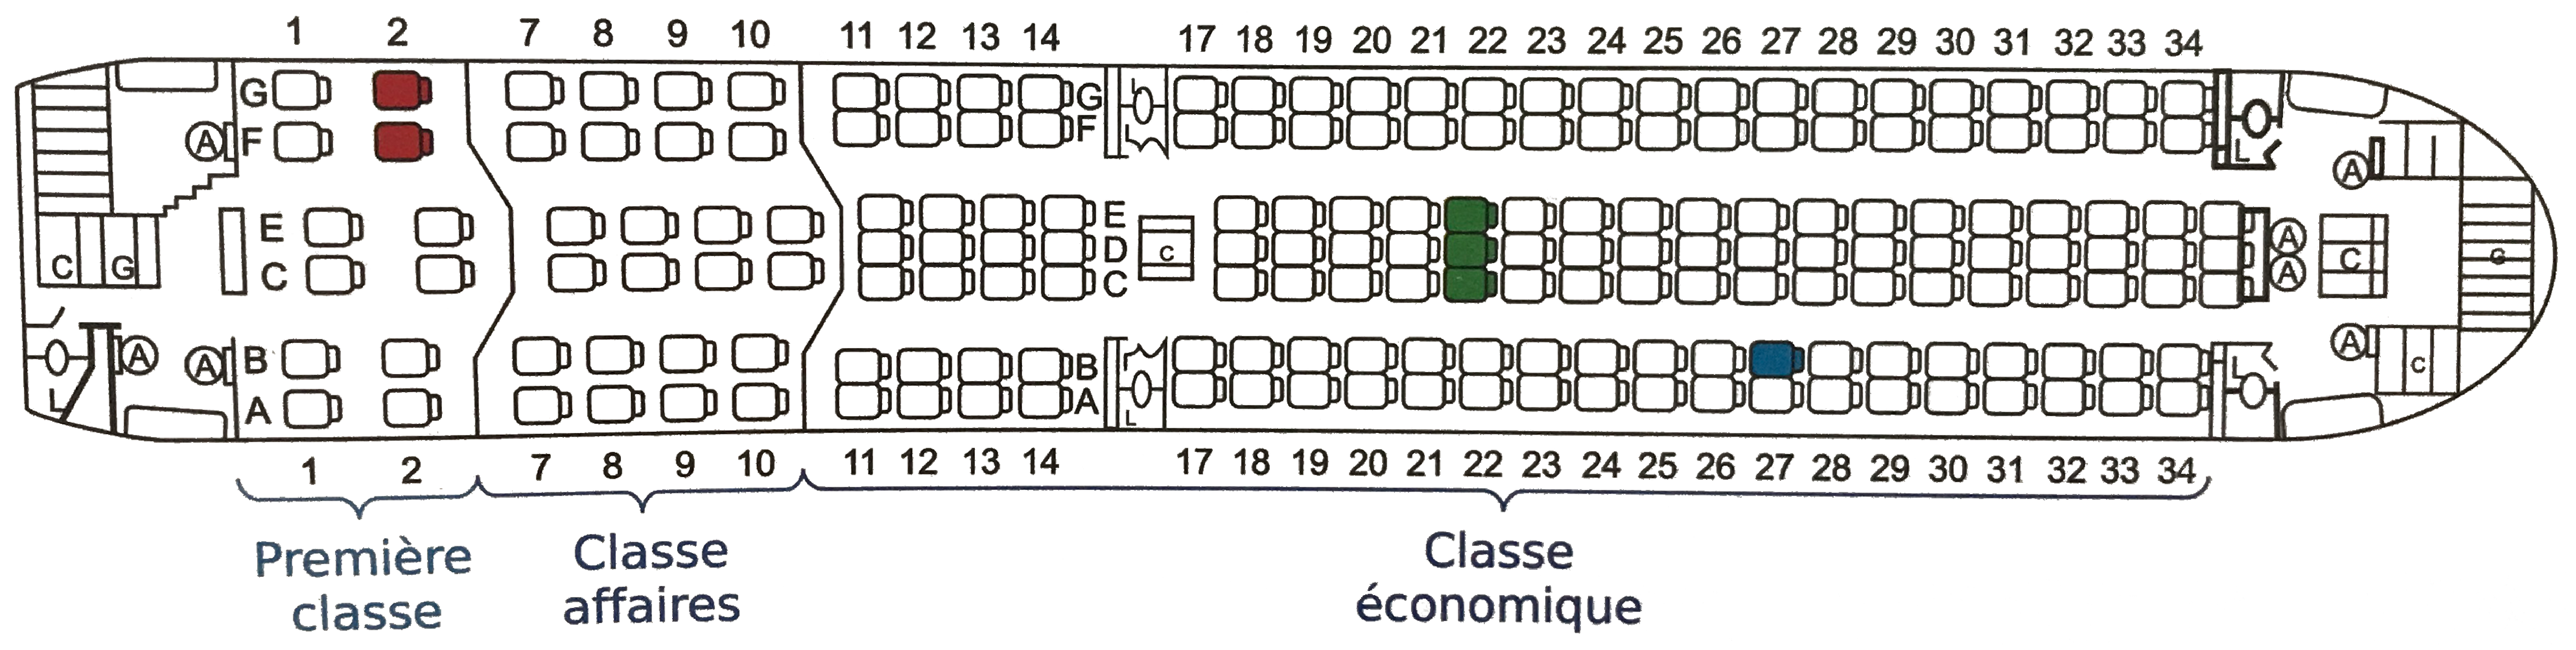
\includegraphics[width=15cm]{boeing}
   \end{center}
   \begin{enumerate}
      \item Indiquer à quelle classe correspond chaque siège : E26 ; E1 ; E7 ; C9 ; B14 ; A34.
      \item Donner la référence des sièges colorés.
      \item Colorier : en rouge les sièges A17 et B17 ; en bleu le siège A1 ; en vert les sièges G29 et F29 ; en noir le siège D12.
   \end{enumerate}
\end{exercice}

\begin{exercice}
   Voici le plan du jardin des plantes de Nantes. \\
  \begin{minipage}{7cm}
      \begin{enumerate}
         \item Combien d'entrées possède ce jardin ?
         \item L'Orangerie se trouve en B1. \\
         Où se trouvent :
         \begin{itemize}
            \item la grande porterie ;
            \item la station de tram ;
            \item la statue Jules Verne ;
            \item la ménagerie ;
            \item le jardin botanique.
         \end{itemize}
         \item Que peut se trouver en :
         \begin{itemize}
            \item C1 ?
            \item D3 ?
            \item C4 ?
            \item B5 ?
         \end{itemize}
         \item Quelles sont les rues qui bordent le jardin des plantes ?
      \end{enumerate}
   \end{minipage}
   \qquad
   \begin{minipage}{9.5cm}
      \includegraphics[width=9.4cm]{jardin}
   \end{minipage}
   \qquad
\end{exercice}

\begin{exercice}
   Voici le plan des trams de l'agglomération de Montpellier : \\ [1mm]
   \begin{minipage}{11.5cm}
      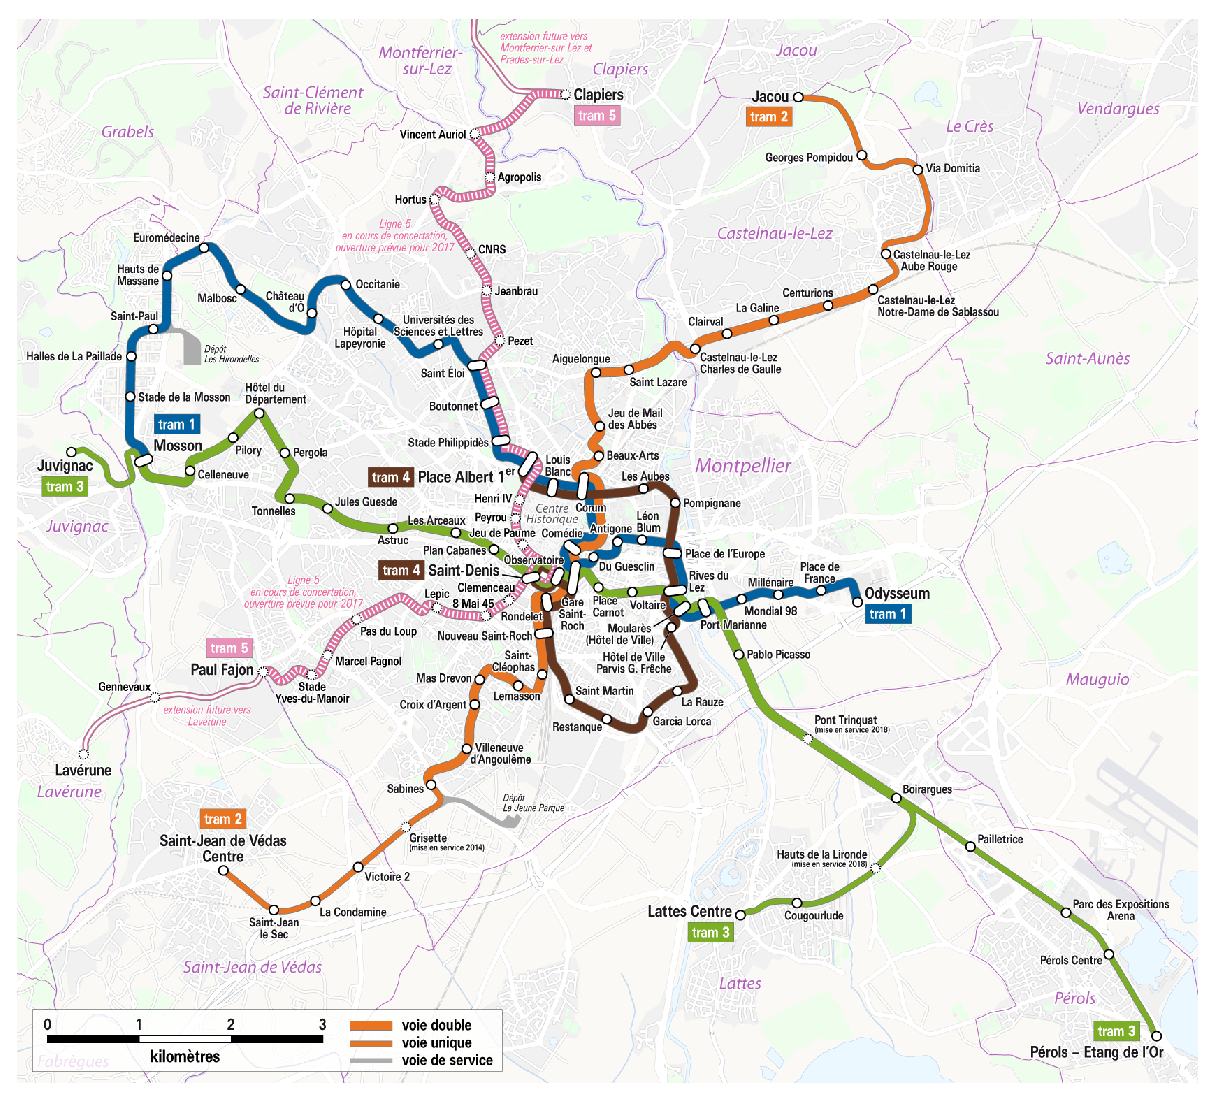
\includegraphics[width=11.5cm]{TAM}
   \end{minipage}
   \quad
   \begin{minipage}{5.5cm}
      \begin{enumerate}
         \item Combien de lignes de tram sont indiquées sur ce plan ?
         \item Combien de lignes de tram sont actuellement en fonctionnement ?
         \item Environ combien de kilomètres mesure la ligne 1 ?
         \item Combien y a-t-il de stations pour la ligne 2 ?
         \item Quelles sont les villes traversées par le ligne 3 ?
         \item Quelle est la particularité de la ligne 4 ?
         \item Quelles sont les deux destinations de la future ligne 5 ?
         \item Quel est l'arrêt le plus proche du collège Simone Veil ?
         \item Vous habitez à Le Crès et souhaitez voir un match de foot au stade de la Mosson. Quel parcours en tram allez-vous effectuer ? 
      \end{enumerate}
   \end{minipage}
\end{exercice}


%%%%%%%%%%%%%%%%%%%%%%%%%%%%%%%%%%%%%%%
%%%%%%%%%%%%%%%%%%%%%%%%%%%%%%%%%%%%%%%
\Recreation

\enigme[La bataille navale]
   \begin{minipage}{5.5cm}  
      \partie[but du jeu.] Faire couler les 5 bateaux de son adversaire.

      \partie[matériel.] Deux grilles composées de 100 cases numérotées horizontalement de 1 à 10 et verticalement de A à J. L'une des grilles sert à disposer ses 5 bateaux et l’autre à marquer les tentatives de localisation des bateaux de l’adversaire. \\  
      {\bf Bateaux à placer} sur la grille :
      \begin{itemize}
         \item 1 porte-avions de 5 cases ;
         \item 1 croiseur de 4 cases ;
         \item 1 contre-torpilleur de 3 cases ;
         \item 1 sous-marin de 3 cases ;
         \item 1 torpilleur de 2 cases.
      \end{itemize}
   
      \partie[règles du jeu.] Les deux joueurs disposent leurs bateaux sur la grille de manière à ce que deux bateaux ne puissent pas être sur des cases adjacentes. \\
      Tour à tour, les joueurs proposent les coordonnées d'un point de la grille en annonçant par exemple \og tir en D8 \fg. L’autre joueur regarde sa grille :
      \begin{itemize}
         \item si un morceau de son bateau s’y trouve, il répond \og touché \fg{} et les deux joueurs marquent cette case d'un cercle ;
         \item si aucun morceau de bateau ne s’y trouve, il répond \og à l'eau \fg{} et les deux joueurs marquent cette case d'une croix ;
         \item si tous les morceaux d’un bateau sont touchés, le joueur dit \og touché-coulé \fg.
      \end{itemize}
      Le premier joueur à couler tous les bateaux de son adversaire gagne.
   \end{minipage}
   \quad
   \begin{minipage}{11cm}
      {\psset{unit=0.95}
      \begin{center}
         \begin{pspicture}(0,0)(11,11)
            \psgrid[gridlabels=0,subgriddiv=0](1,0)(11,10)
            \rput(0.5,0.5){J}
            \rput(0.5,1.5){I}
            \rput(0.5,2.5){H}
            \rput(0.5,3.5){G}
            \rput(0.5,4.5){F}
            \rput(0.5,5.5){E}
            \rput(0.5,6.5){D}
            \rput(0.5,7.5){C}
            \rput(0.5,8.5){B}
            \rput(0.5,9.5){A}
            \rput(0.5,1){\multido{\n=1+1}{10}{\rput(\n,9.5){\n}}}
         \end{pspicture}
      \end{center}
      \begin{center}
         \begin{pspicture}(0,0)(11,11)
            \psgrid[gridlabels=0,subgriddiv=0](1,0)(11,10)
            \rput(0.5,0.5){J}
            \rput(0.5,1.5){I}
            \rput(0.5,2.5){H}
            \rput(0.5,3.5){G}
            \rput(0.5,4.5){F}
            \rput(0.5,5.5){E}
            \rput(0.5,6.5){D}
            \rput(0.5,7.5){C}
            \rput(0.5,8.5){B}
            \rput(0.5,9.5){A}
            \rput(0.5,1){\multido{\n=1+1}{10}{\rput(\n,9.5){\n}}}
         \end{pspicture}
      \end{center}}
   \end{minipage}

